\section{Durchführung}
\label{sec:Aufbau}
Als erste Messreihe wird die Charakteristik des Zählrohres aufgenommen.
Dabei werden die Impulse pro $\SI{60}{\sec}$ bei einer
Spannung zwischen $\SI{300}{\volt}$ und $\SI{700}{\volt}$ gemessen,
sowie die jeweilige Stromstärke.

Im Versuchsaufbau, vgl Abbildung \ref{fig:versuchsaufbau}, wird die Stromstärke
an einem im Zählrohr eingebauten Amperemeter abgelesen.
Oszilloskop und Zählwerk, samt Verstärker, sind über einen Y-Stecker direkt am
Zählrohr über Koaxialkabel angeschlossen.

\begin{figure}
    \centering
    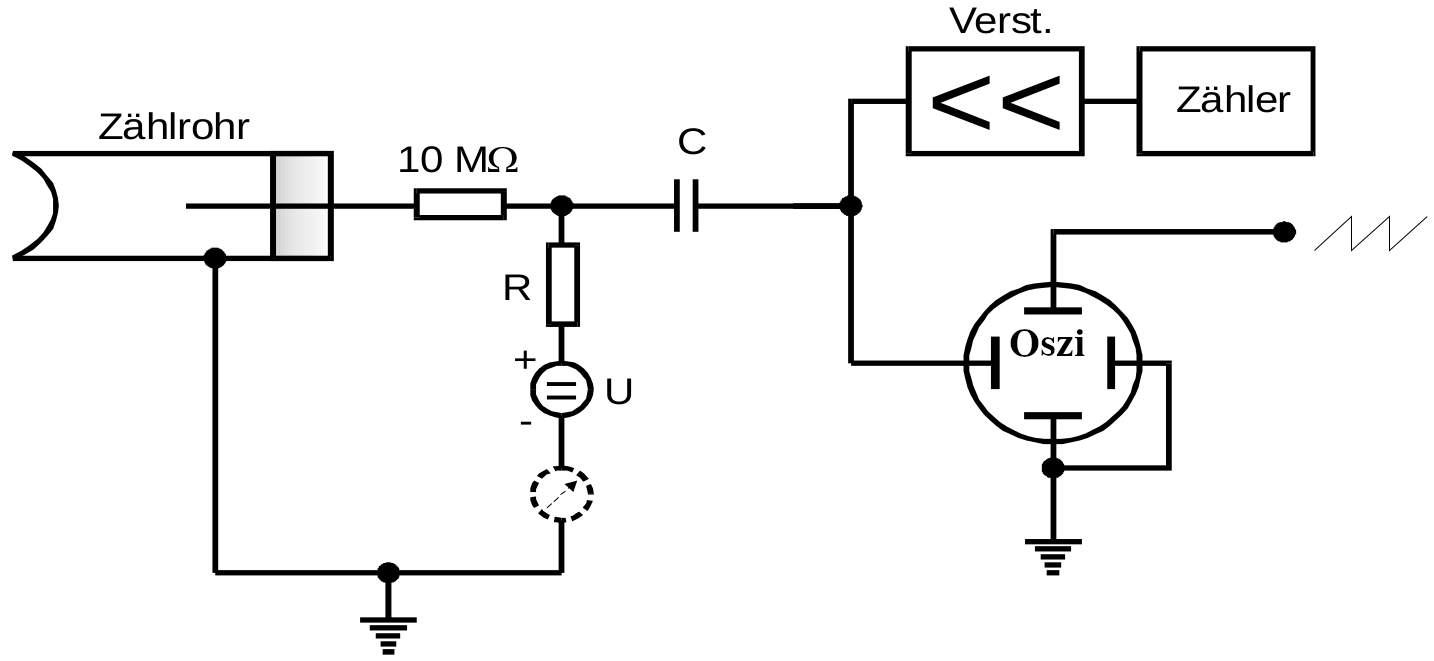
\includegraphics[width=0.7\paperwidth]{content/aufbau.png}
    \caption{Skizze des Versuchsaufbaus. \cite{Anleitung}}
    \label{fig:versuchsaufbau}
\end{figure}

Im Anschluss werden mithilfe des Oszilloskops
die Impulse als Funktion der Zeit auf dem Schirm sichtbar gemacht und für fünf
verschiedene Spannungen die Totzeit ausgelesen.
Die Nachentladungszeit wird für 4 Spannungen, im Bereich des Plateaus, bestimmt.

Als letztes wird die Zwei-Quellen-Methode durchgeführt (siehe \ref{sec:zweiquellen}).
Es wird in der Reihenfolge $N_1, N_{1,2}, N_2$ gemsssen, um die Abstände zwischen
Quellen und Zählrohr gleich zu lassen.
